\documentclass[slovak, master]{diploma}

% Packages (balíky makier)
\usepackage[autostyle=true, czech=quotes]{csquotes} % korektná sadzba úvozoviek, podpora pre balík biblatex
\usepackage[backend=biber, style=iso-numeric, alldates=iso]{biblatex} % bibliografia
\usepackage{dcolumn} % stĺpce tabuľky s číselnými hodnotami
\usepackage{subfig} % makrá pre "podobrázky" a "podtabuľky"
\usepackage[csharp]{diplomalst} % sádzanie
\usepackage{svg}
%\usepackage[python]{diplomalst}
%\usepackage{tcolorbox} % oramovanie

% ------------------------------------------------------

% Definované vlastné metódy, triedy a príslušné farby
% viz bakalarka

% ------------------------------------------------------

% Nový druh tabuľkového stĺpca, v ktorom sú čísla zarovnané podľa desetinnej čiarky
%\newcolumntype{d}[1]{D{,}{,}{#1}}

% Odstranenie warningov s underfull vbox
%\raggedbottom

% Nastavenie tex color boxu
%\newtcbox{\mybox}[2][black]{outer arc=0pt,  boxsep=0pt, left=0pt, right=0pt, top=0pt, bottom=0pt, boxrule=2pt}

% ------------------------------------------------------

%Zásady pro vypracování
% S umělou inteligencí, která je zodpovědná za rozhodování, se setkáme ve většině počítačových her, ať už jde o hry deskové, plošinové nebo např. tahové. Cílem této diplomové práce je naimplementovat herní prostředí, v němž budou pro rozhodování použity klasické algoritmy jako např. ID3, C4.5, CART (regresní stromy), CHAID (Chi-square, automatic interaction detection), MARS ( (multivariate adaptive regression splines), náhodný les (random forest) a algoritmy jako Deep Q-learning, Double Deep Q-learning, popř. hluboké neuronové sítě a tyto metody porovnat na základě experimentů a následné statistické analýzy. Metody budou porovnány na základě výkonu a úspěšnosti z hlediska řešení daných problémů.

% Zásady pro vypracování:
% 1. Seznamte se s algoritmy jmenovanými výše a způsobem jejich použití v počítačových hrách.
% 2. Navrhněte vlastní netriviální počítačovou hru, kde budou vybrané algoritmy použity pro rozhodování tzv. NPC (non-playing character). Při výběru algoritmů je potřeba, aby byly zastoupeny obě kategorie výše zmíněných algoritmů - tzn. klasické i algoritmy strojového učení. Celkem by mělo být použito aspoň 5 algoritmů, kde aspoň 2 budou patřit do kategorie strojového učení. Ve hře bude implementována postava hráče, který bude proti NPC bojovat.
% 3. Naimplementujte zvolené algoritmy a proveďte jejich srovnání na základě opakovaných experimentů. Během implementace klaďte důraz na efektivitu. Žádný z algoritmů nesmí být proti jinému zvýhodněn. Proveďte statistickou analýzu a s použitím vhodných statistických testů vyhodnoťte kvalitu poskytovaného řešení těchto algoritmů a jejich výkon.
% 4. Výsledky zpracujte v podobě tabulek a grafů a na jejich základě proveďte vyhodnocení testů. Shrňte výhody a nevýhody jednotlivých algoritmů. V závěru uveďte, který algoritmus dosáhl nejlepšího výkonu a který byl při řešení daných úkolů nejúspěšnější.

% ------------------------------------------------------

% Titulná strana
\ThesisAuthor{Bc. Miroslav Kačeriak}
\ThesisSupervisor{prof. Ing. Jan Platoš, Ph.D.}
\CzechThesisTitle{Rozhodování v počítačových hrách - srovnání metod umělé inteligence}
\EnglishThesisTitle{Decision Making in Computer Games - a Comparison of Artificial Intelligence Methods}
\ThesisAssignmentFileName{ThesisSpecification_KAC0067_vsboee22026009.pdf}
\SubmissionYear{2023}

% ------------------------------------------------------

% Abstrakty
\CzechAbstract{TODO}

\CzechKeywords{spätnoväzobné učenie, rozhodovacie stromy, ID3, D4.5, CART, Unity engine, C\#, Python}

\EnglishAbstract{TODO}

\EnglishKeywords{reinforcement learning, decision trees, ID3, D4.5, CART, Unity engine, C\#, Python}

% ------------------------------------------------------

% Poďakovanie
\Acknowledgement{Rád by som na tomto mieste poďakoval prof. Ing. Jánovi Platošovi, Ph.D. za pomoc a ochotu prejavenú popri vedení tejto diplomovej práce a mojej priateľke Zdenke za trpezlivosť a prínosné rady, bez ktorých by výsledná práca bola o niečo chudšia.}

% ------------------------------------------------------

% Skratky
\AddAcronym{AI}{Artificial intelligence}
\AddAcronym{API}{Application Programming Interface}
\AddAcronym{CART}{Classification and Regression Tree}
\AddAcronym{GUI}{Graphic User Interface}
\AddAcronym{FPS}{Frames Per Second}
\AddAcronym{NPC}{Non-Playable Character}
\AddAcronym{UI}{User Interface}

% ------------------------------------------------------

% Literatúra
\addbibresource{literature.bib}

% ------------------------------------------------------

% Samotný dokument
\begin{document}
\MakeTitlePages

% Zoznam obrázkov
\listoffigures
\clearpage

% Zoznam tabuliek
\listoftables
\clearpage

% Zoznam zdrojakov
\lstlistoflistings
\clearpage

% Chapter 1
\chapter{Úvod}
\label{sec:Introduction}
%TODO

% ------------------------------------------------------

% Teória
% Chapter 2
\chapter{Umelá inteligencia v hrách}
\label{sec:AI in games}
%TODO

\section{Rozhodovacie stromy}
\label{sec:DecisionTreesOverview}

\section{Strojové učenie}
\label{sec:MachineLearningOverview}
%TOOD
\subsection{Spätnoväzobné učenie}
\label{sec:ReinforcemenLearningOverview}
%TODO

% ------------------------------------------------------

% Vypracovanie
% Chapter 3
\chapter{Použité technológie}
\label{sec:Tech}
%TODO
\section{Unity Engine}
\label{sec:Unity}
%TODO
\section{Nástroj ML-Agents}
\label{sec:ML-Agents}
%TODO
%...?

% Chapter 4
\chapter{Hra a herné prostredie}
\label{sec:GameOverview}
Táto kapitola je venovaná vytvorenej hre, všetkým jej aspektom a princípom fungovania. Prvá sekcia si kladie za cieľ popísať žánrové a príbehové zasadenie hry. V ďalších sekciách je potom podrobne prebratá architektúra a fungovanie jednotlivých herných mechaník, s dôrazom na zmyslové vnímanie jednotlivých NPC agentov.

\section{Žáner a príbehové zasadenie}
\label{sec:GenreAndSetting}
Hra samotná má svojou hrateľnosťou najbližšie k žánru stealth. Tento žáner sa vyznačuje tým, že hráč sa snaží vyhnúť odhaleniu a následnému priamemu stretu s nepriateľom. K dosiahnutiu cieľa je teda využívaný pomalý a tichý postup, kde každý krok by mal byť dobre premyslený a načasovaný. 

Príbeh hry je zasadený do pirátskeho prostredia. Hráč sa ocitá v roli radového člena pirátskej posádky, ktorá bola napadnutá flotilou anglického námorníctva. S vypätím všetkých síl sa mu na poškodenom záchrannom člne podarilo dostať na najbližší obývaný ostrov, kde však zisťuje, že nie je všetko v poriadku. Namiesto obyvateľov ostrova nachádza len agresívnych kostlivcov. 

Hráčovou úlohou je nájsť na ostrove funkčný čln, pozbierať zásoby nutné na ďalšiu plavbu a pokiaľ možno pri tom nevzbudiť pozornosť.

\begin{figure}[!htbp]
	\centering
	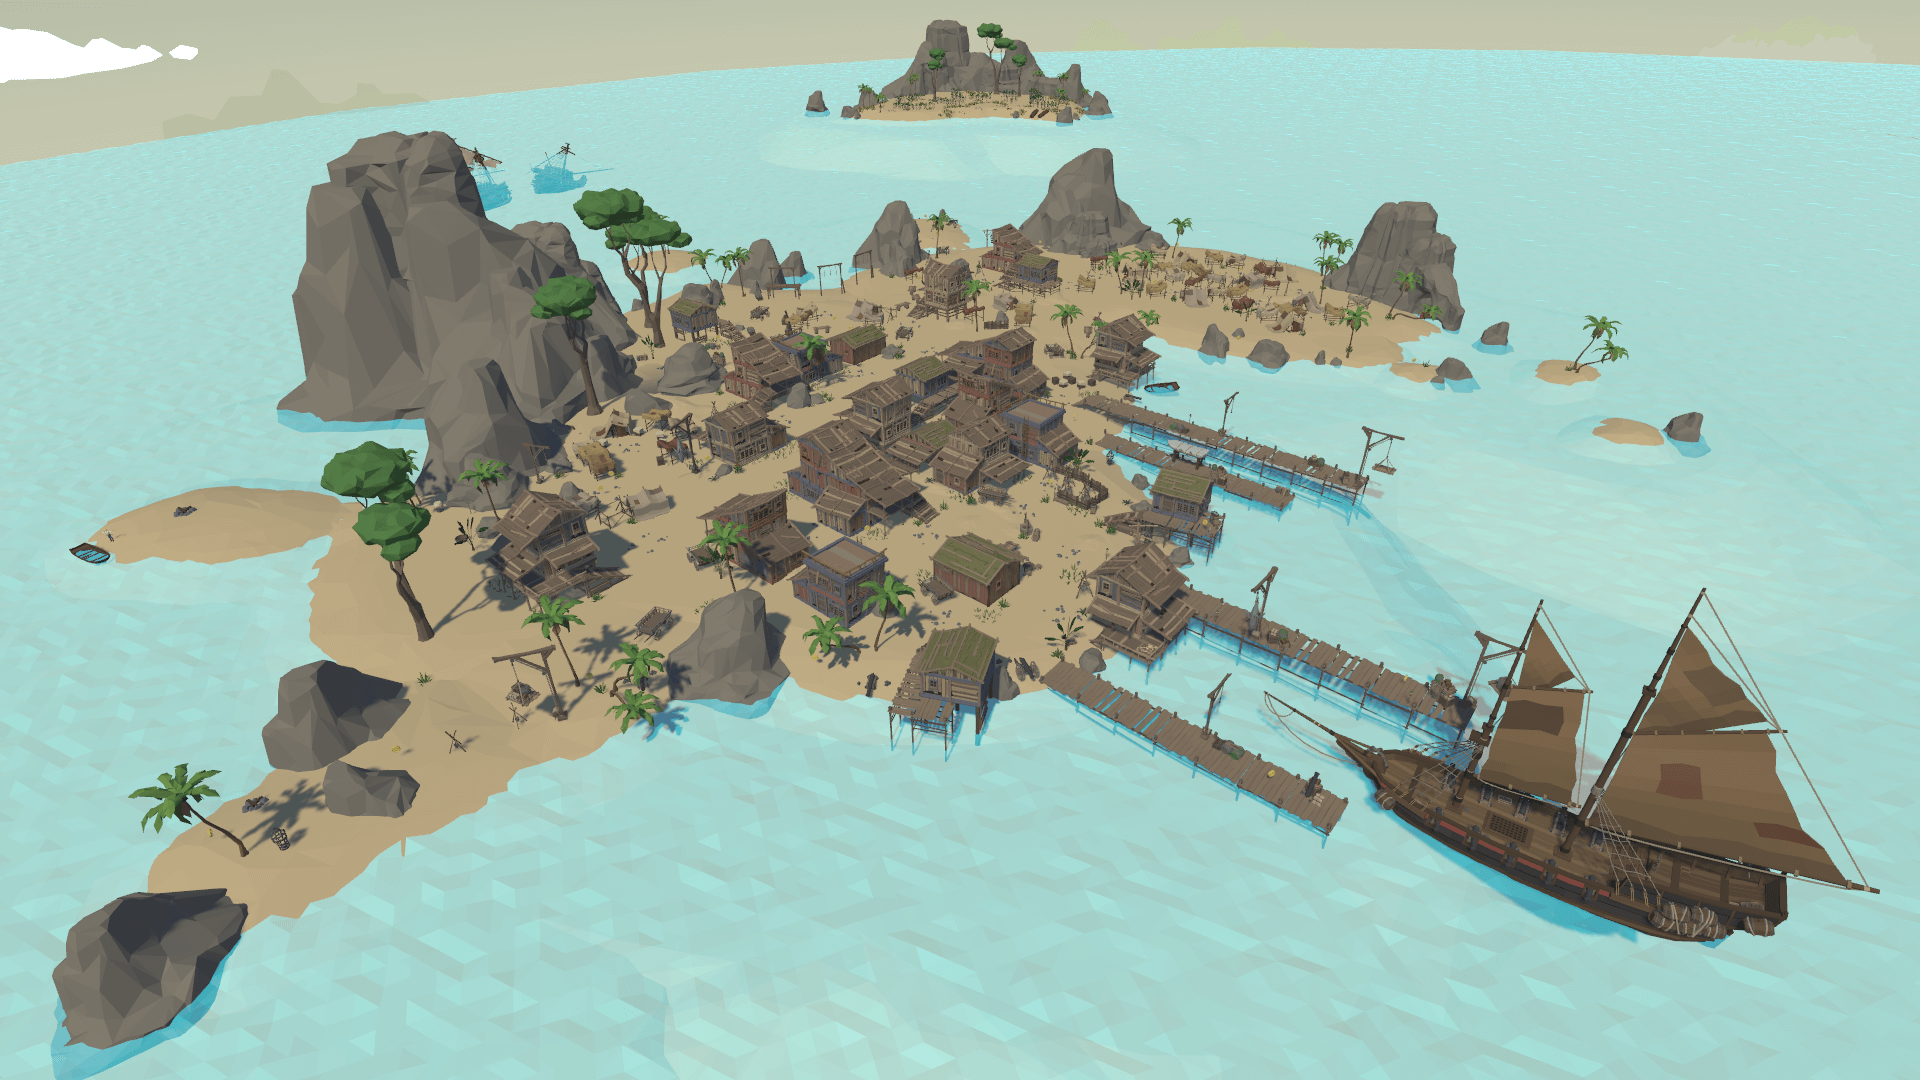
\includegraphics[width=.9\textwidth]{Figures/game_compressed.png}
	\caption{Vyrenderovaná snímka z hry}
	\label{pic:GameScreenshot}
\end{figure}

\section{Architektúra hry}
\label{sec:GameStructure}
%TODO
%spomenut synty tu
%manazeri overview
Hra je rozdelená do dvoch samostatných scén. Konkrétne ide o hlavnú scénu, kde sa odohráva samotná herná slučka a scénu s hlavnou ponukou. V editore Unity je možné medzi jednotlivými scénami ľubovoľne prepínať, prípadne mať aktívnych niekoľko scén naraz. V samostatnom zostavení aplikácie je však nutné vybrať, ktoré konkrétne scény budú prítomné. Každá scéna potom dostane poradové číslo, tzv. build index a scéna s číslom nula, v tomto prípade hlavná ponuka, bude spustená ako prvá. Scéna s hlavnou ponukou je bližšie popísaná v sekcií \ref{sec:MainMenuAndUI}.

Scénu je potom možné chápať ako koreňový adresár pre hierarchiu objektov v hre. Jednotlivé herné objekty je možné vložiť do scény priamo alebo ako potomka iného herného objektu. Manipulácia s pozíciou, rotáciou či mierkou objektu sa teda aplikuje aj na všetkých jeho potomkov. Naopak to však neplatí. Z tohto dôvodu sa rozlišujú dve súradnicové sústavy, a síce globálna (celková) a lokálna (relatívna voči predkovi). Využitie globálnej súradnicovej sústavy však vyžaduje vziať do úvahy parametre všetkých predkov daného objektu v scéne, čo nie je ideálne z hľadiska výkonu. Preto bol v projekte preferovaný lokálny súradnicový systém napríklad u herných NPC agentov či predmetov, ktoré je v hre možné zbierať a je pre nás zaujímavá ich pozícia. Predkovia týchto objektov sú potom umiestnení v počiatku súradnicovej sústavy, čo zaisťuje konzistenciu so zvyškom objektov v scéne.

V každej scéne sa nachádza objekt MainManager, ktorý slúži ako prístupový bod k ostatným manažérom, ktorí spravujú centrálne prvky hry. Tento typ architektúry sa kvôli svojej jednoduchosti často uplatňuje medzi malými až strednými projektami. V tomto projekte sú použité objekty ConfigManager, GameManager, InputManager a SoundManager, nie všetky sú však vyžadované v oboch scénach. 

Krátky popis jednotlivých manažérov:
\begin{itemize}
  \item \textbf{ConfigManager} -- je prístupovým bodom k nastaveniam hry, zaisťuje serializáciu a deserializáciu dát, rovnako ako ich perzistentnosť po každej zmene.
  \item \textbf{GameManager} -- reštartuje scénu pri smrti alebo výhre hráča, kontroluje prerekvizity výhry, aktualizuje grafické užívateľské rozhranie pri získaní predmetu a zobrazuje kontextovú ponuku na ukončenie hry či návrat do hlavnej ponuky po stlačení príslušnej klávesy.
  \item \textbf{InputManager} -- je abstrakciou nad konkrétnou implementáciou získavania vstupu z klávesnice, myši, či iných herných periférií, čo umožňuje na jednom centrálnom mieste zamieňať tzv. starý input systém za nový, či naopak, prípadne z testovacích dôvodov hráčsky vstup úplne ignorovať. 
  \item \textbf{SoundManager} -- Vyvoláva jednoduchú simuláciu zvuku, na ktorú môžu zareagovať NPC agenti v dosahu.
\end{itemize}

\subsection{Herná slučka}
\label{sec:GameLoop}
Tradičná herná slučka definovaná napríklad podľa \cite{GameAlgorithms} sa skladá z troch fáz:

\begin{enumerate}
  \item Spracovanie vstupov
  \item Aktualizácia herného sveta
  \item Generovanie výstupov
\end{enumerate}

Hra teda prijme užívateľský vstup, na základe neho aktualizuje herný svet (dynamické objekty, ktoré sa v ňom vyskytujú) a výsledný stav je potom vyrenderovaný hráčovi v ďalšom snímku. Tento postup sa opakuje niekoľkokrát za sekundu, čo vyvoláva ilúziu dynamického sveta. Dnes sa považuje za štandard aktualizácia hernej slučky 30 až 60 krát za sekundu. Dnešný hardvér však už podporuje vykresľovanie aj o rýchlosti 500FPS. Ako lepšia metrika pre herných vývojárov sa však používa tzv. frame time, teda trvanie jednej hernej slučky v ms.

\begin{figure}[!htbp]
	\centering
	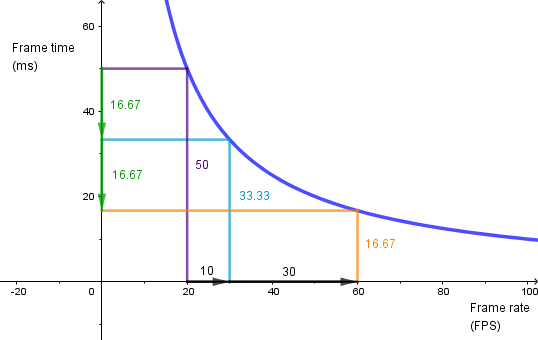
\includegraphics[width=.9\textwidth]{Figures/frameTimeVsFPS.png}
	\caption{Metriky Frame Time a FPS \cite{FrameTimeFPS}}
	\label{pic:FrameTimeFPS}
\end{figure}

V kontexte konkrétnej hry sa však pojem herná slučka alebo základná herná slučka (core game loop) využíva skôr na popis základných herných mechaník. V tomto prípade by teda šlo o prechod z bodu A do bodu B a zozbieranie určitého počtu predmetov na vymedzenej hernej ploche.

Pokiaľ hráčovi klesne život na nulu, hra pre neho končí a vracia sa na počiatočnú lokáciu. Nepriatelia a zbierateľné predmety sa vrátia na svoje počiatočné pozície. Ak hráč dôjde do cieľa a splní podmienku, že má v inventári určitý počet predmetov daného typu, hru vyhráva. 

V hre je možné nastaviť typ umelej inteligencie NPC agentov. Jednotlivé možnosti sú popísané v nasledujúcich sekciách.

Základnú hernú slučku obstaráva objekt GameManager popísaný v sekcií \ref{sec:GameStructure}. Po hernej ploche je ručne rozmiestnených päť fliaš, z ktorých musí hráč nájsť a zobrať aspoň tri a tridsaťpäť mincí, pričom je pre dosiahnutie výhry nutné mať aspoň dvadsaťpäť. 

Oba typy objektov dedia z triedy Pickup vo výpise \ref{src:Pickup}. Tá potom dedí priamo z triedy UnityEngine.MonoBehaviour, čo je bázová trieda, z ktorej dedia musia dediť všetky triedy, ktoré nejakým spôsobom využívajú Unity API. Typicky ide o metódy ako napríklad Awake(), Start(), Update(), či FixedUpdate(), ktoré sú definované v životnom cykle Unity objektu, ale aj metódy sprístupňujúce prácu s korutinami apod.
\vspace{8pt}
\begin{lstlisting}[label=src:Pickup,caption={Trieda Pickup slúžiaca ako predok všetkých zberateľných predmetov v hre}]
public class Pickup : MonoBehaviour
{
    public event Action<Pickup> OnPickedUp;
    private WaitForEndOfFrame waitForFrameToEnd = new WaitForEndOfFrame();
    private MeshRenderer mesh;

    private void Start() 
    {
        MainManager.Instance.GameManager.RegisterPickup(this);
        mesh = GetComponentInChildren<MeshRenderer>();
    }
    private void OnTriggerEnter(Collider other) 
    {
        if (!other.gameObject.CompareTag(Constants.PlayerTag))
            return;

        OnPickedUp?.Invoke(this);
        StartCoroutine(LerpPosition(transform.position, Camera.Instance.PickupTarget.position, 0.2f, () => { gameObject.SetActive(false); }));
    }
    private void OnDestroy() 
    {
        MainManager.Instance.GameManager.UnregisterPickup(this);
    }
    IEnumerator LerpPosition(Vector3 start, Vector3 end, float timeToMove, Action callback) 
    {
        float time = 0;

        while (time < 1)
        {
            mesh.transform.position = Vector3.Lerp(start, end, time);
            time += Time.deltaTime / timeToMove;

            yield return waitForFrameToEnd;
        }

        mesh.transform.position = end;
        callback();
    }
}
\end{lstlisting}

V metóde Start(), teda na začiatku svojho životného cyklu, po spustení scény sa každý zberateľný objekt zaregistruje v objekte GameManager, čo spôsobí napojenie na event OnPickedUp, a umožní GameManagerovi v správnej chvíli zareagovať na získanie predmetu hráčom a aktualizovať GUI či inventár bez nutnosti periodického dotazovania. Nakoľko je v tomto evente odosielaná aj daná inštancia objektu je jednoduché zistiť o aký typ predmetu ide.

Metóda OnTriggerEnter() je potom zavolaná v momente, keď hráčov kontroler začne kolidovať s box colliderom daného objektu. K tomu je nutné nastaviť tento box collider ako trigger a zároveň mať na objekte prítomnú komponentu rigidbody, ktorá sa stará o spracovanie fyziky na objekte. V tomto momente sa zároveň pomocou korutiny LerpPosition() začne objekt rýchlo pohybovať do pravého horného rohu obrazovky, kde sa nachádza UI element ukazujúci hráčovi počet zozbieraných predmetov, a následne sa deaktivuje. Tento efekt bol často využívaný v starších 2D platformových hrách. Zberateľný predmet mincu spolu s vizuálnym efektom je možné vidieť na obrázku \ref{pic:Pickup}.

\begin{figure}[!htbp]
	\centering
	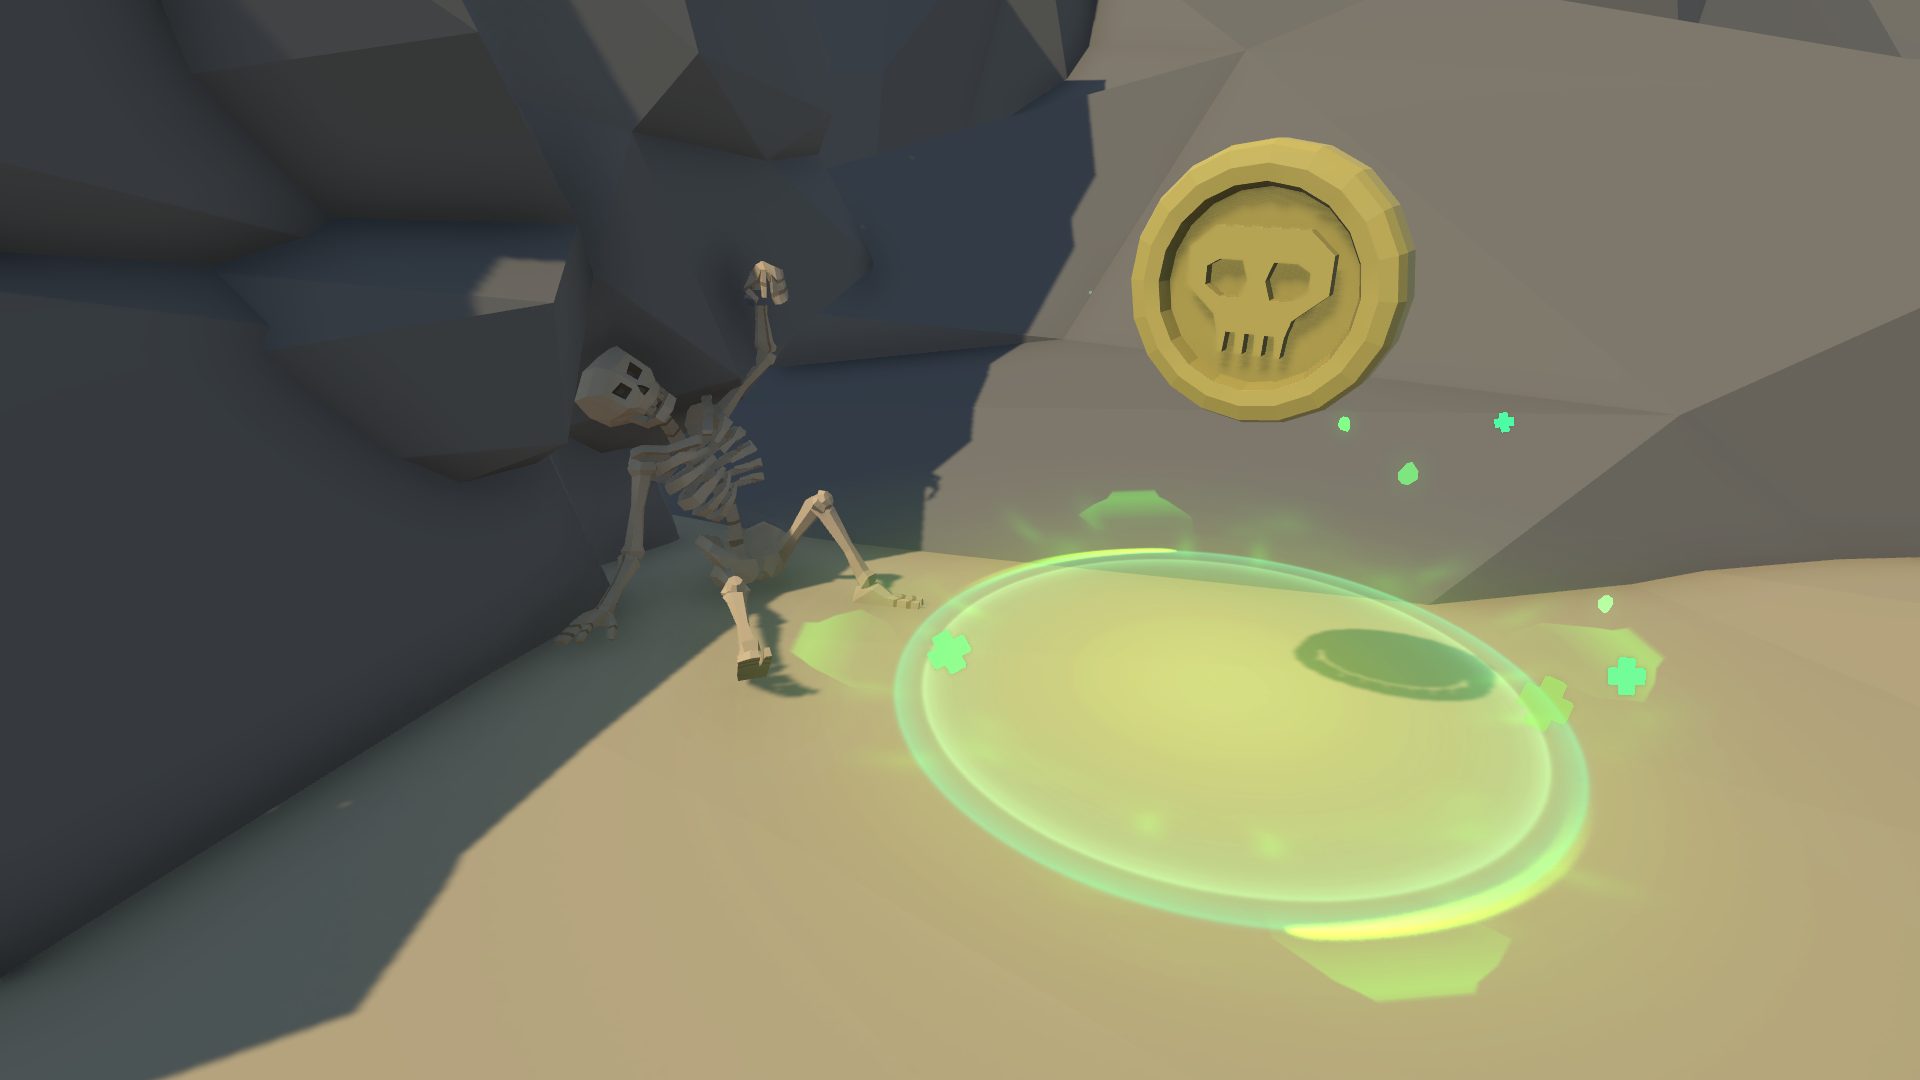
\includegraphics[width=.9\textwidth]{Figures/pickup.png}
	\caption{Zberateľný predmet minca}
	\label{pic:Pickup}
\end{figure}

Väčšina informácií týkajúcich sa zberateľných predmetov sa vzťahuje aj na objekt Finish, ktorého úlohou je ukončiť hru v prípade, že s ním hráčov kontroler začne kolidovať. Musí teda obsahovať komponentu box collider nastavenú ako trigger a komponentu rigidbody. Pri štarte hry sa tento Finish rovnako ako zberateľné predmety zaregistruje pod GameManagera a v metóde OnTriggerEnter(), po overení, že naozaj koliduje s hráčom vyvolá event OnTriggered. Nakoľko bol Finish využívaný aj v trénovacej fáze, bol pre tento účel vytvorený jednoduchý interface IFinish zobrazený vo výpise \ref{src:IFinish} a jeho dve implementácie: FinishGame a FinshEpisode. Prvá spomínaná je využívaná v hlavnej scéne a ukončuje hru, druhá, ako názov napovedá, ukončuje trénovaciu epizódu v neprospech AI agenta. Jednotlivé trénovacie scenáre sú popísané v sekcií \ref{sec:Training}.

\vspace{8pt}
\begin{lstlisting}[label=src:IFinish,caption={Interface IFinish}]
public interface IFinish
{
    public event Action OnTriggered;
}
\end{lstlisting}

Po vyvolaní spomínaného eventu GameManager overí prerekvizity výhry a pokiaľ ich hráč spĺňa ukončí hru. Tento postup je možné vidieť vo výpise \ref{src:FinishGame}. Event OnGameFinished zároveň všetkým odberateľom oznámi ukončenie hry. Najdôležitejší odberatelia eventu sú herná kamera a pohybový systém hráča, ktorí okamžite zastavia svoju činnosť a stanú sa pasívnymi. Zároveň s týmto sa hráčovi začne animovane zobrazovať informácia o úspešnom dokončení hry a po nejakej sa dobe reštartuje scéna, čo umožní hráčovi skúsiť to znova napríklad s inými parametrami.

\vspace{8pt}
\begin{lstlisting}[label=src:FinishGame,caption={Ukončenie hry v prípade výhry hráča}]
private bool PrerequisitesMet()
{
    return (pickedBottles >= minBottles) && (pickedCoins >= minCoins);
}
private void GameFinished()
{
    if (!PrerequisitesMet())
    {
        ShowPrerequisitesNotMetInfo();
        return;
    }

    OnGameFinished?.Invoke();

    if (youWonUI != null)
        youWonUI.SetActive(true);

    StartCoroutine(RestartSceneCoroutine());
}
private IEnumerator RestartSceneCoroutine()
{
    yield return uiWait;
    SceneManager.LoadScene(SceneManager.GetActiveScene().name);
}
\end{lstlisting}

\begin{figure}[!htbp]
	\centering
	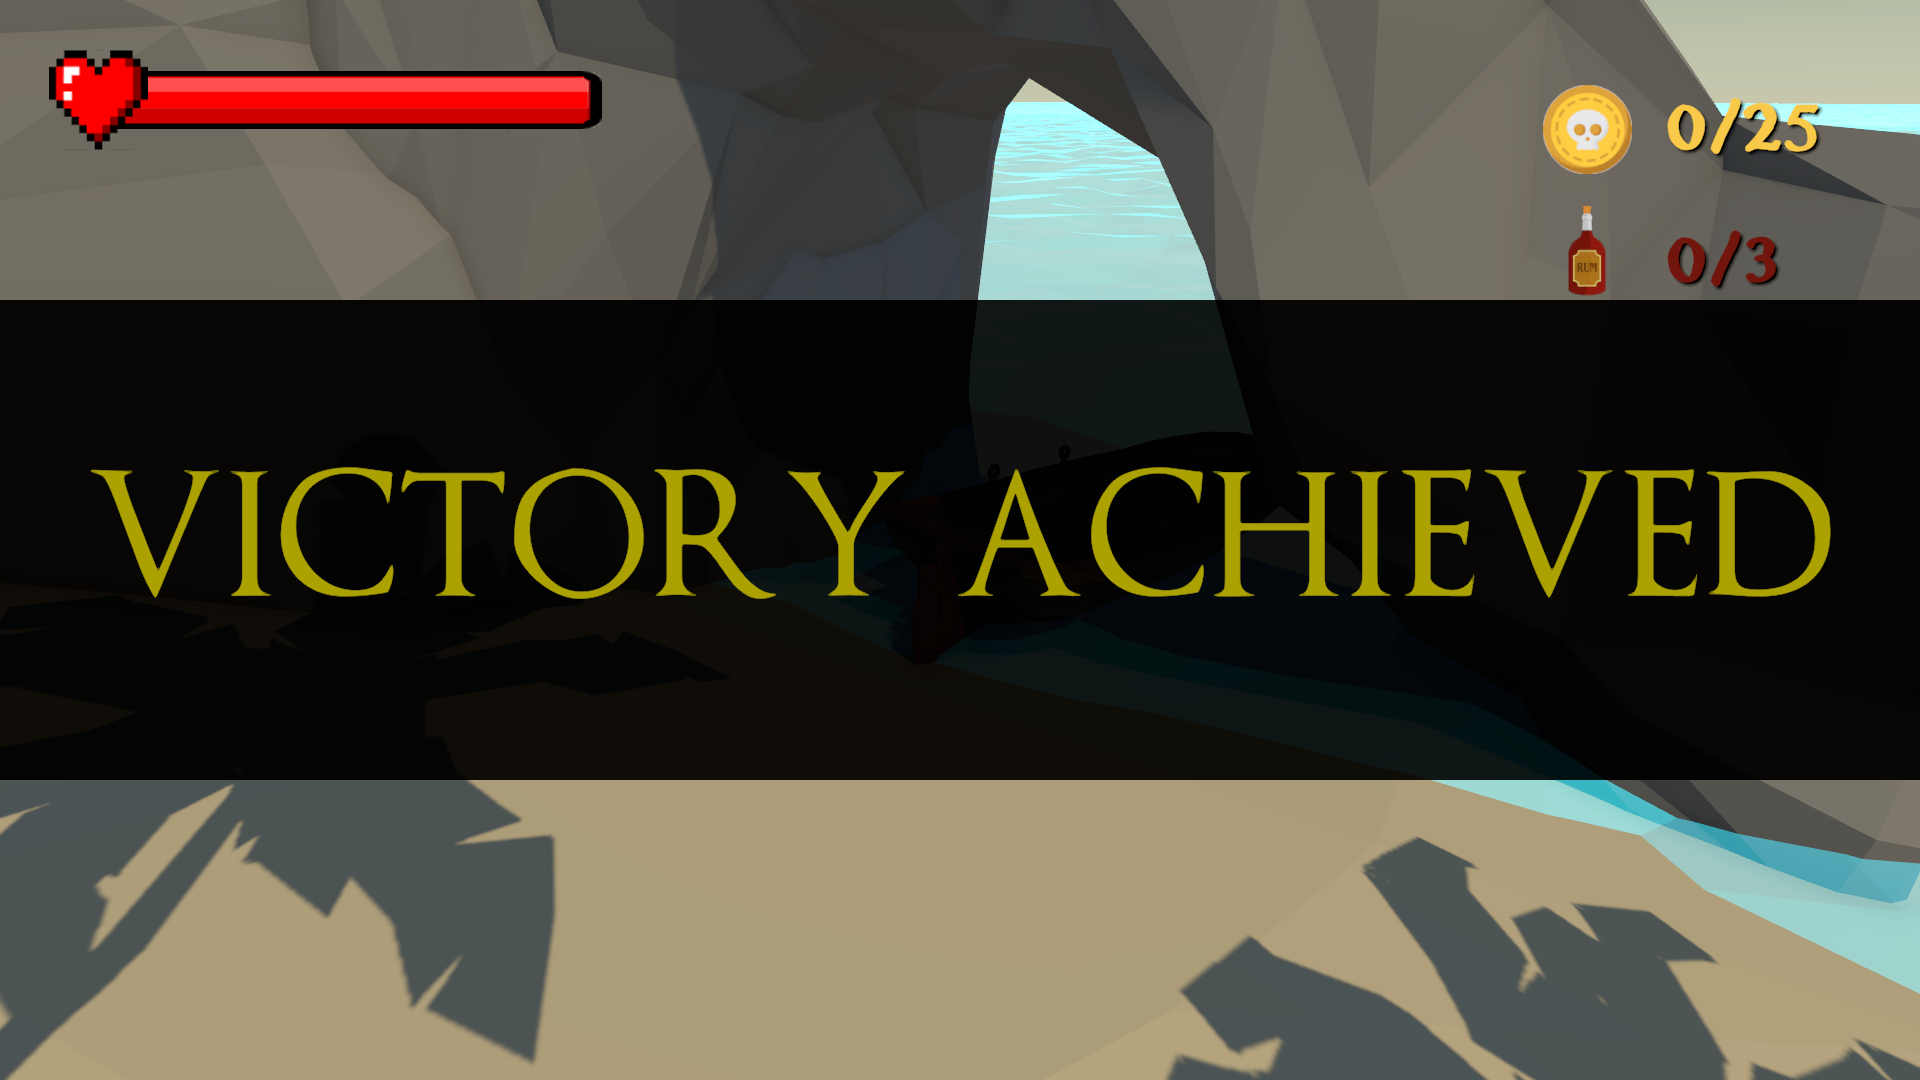
\includegraphics[width=.9\textwidth]{Figures/finishing.png}
	\caption{UI obrazovka oznamujúca hráčovi úspešné dokončenie hry}
	\label{pic:Pickup}
\end{figure}

Medzi ďalšie kompetencie GameManagera patrí na základe nastavení uložených v ConfigManagerovi inštancovať pri štarte hry NPC agentov určeného typu na konkrétne pozície a rotácie, čo je znázornené vo výpise \ref{src:GameManOnStart}. Viac o štruktúre agentov, ich inštancovaní a fungovaní je popísané v sekcií \ref{sec:Agents}.

\vspace{8pt}
\begin{lstlisting}[label=src:GameManOnStart,caption={Inštancovanie NPC agentov na základe nastavení}]
public void OnStart() 
{
    if (!spawner)
        return;

    var controllMethod = MainManager.Instance.ConfigManager.NPCControll;

    if (controllMethod == ENPCControllMethod.DecisionTrees)
        spawner.SpawnRegularEnemies();
    else if (controllMethod == ENPCControllMethod.ReinforcementLearning)
        spawner.SpawnMLEnemies();
    else
        throw new Exception("Invalid NPC controll method");
}
\end{lstlisting}

Vo výpise \ref{src:GameManOnStart} je možné si povšimnúť, že pre využitie možností životného cyklu objektu nie je využitá metóda Start() ale vlastná metóda OnStart(), ktorá je volaná z metódy Start() objektu MainManager. Tento postup je využitý z dôvodu lepšieho výkonu, nakoľko stačí z natívneho C++ kódu volať určitú metódu životného cyklu iba na jednom hlavnom objekte a ten sa postará o volanie vo zvyšných objektoch, ktoré spravuje. Tento postup je opäť často využívaný v rámci optimalizácie projektu. Ďalšou výhodou je však aj možnosť riadiť poradie, v akom budú metódy zavolané na konkrétnych objektoch a nenechávame to na rozhodnutí herného enginu. 

Aby mohol teda GameManager získať dáta z ConfigManagera musíme sa uistiť, že jeho inicializácia už prebehla a v tomto prípade boli deserializované potrebné dáta z perzistentného úložiska nastavení. 

Poslednou kompetenciou GameManagera je periodicky v rámci hernej slučky zisťovať od objektu InputManager, či bola stlačená klávesa na pozastavenie hry a na základe toho zobraziť hráčovi ponuku, či chce ukončiť hru alebo sa vrátiť do hlavnej ponuky. Tento postup je demonštrovaný vo výpise \ref{src:GameManOnUpdate} a bol zvolený z dôvodu, že natívny input systém enginu Unity nedokáže spracovávať užívateľský vstup eventovým prístupom. Event OnPauseMenuVisibilityChanged potom upozorní odberateľa (hernú kameru) aby nereagoval na hráčov vstup, nakoľko prioritnejšou úlohou sa stal výber akcie, ktorá sa má vykonať. Zobrazenú ponuku akcií je možné vidieť na obrázku \ref{pic:PauseUI}.

\vspace{8pt}
\begin{lstlisting}[label=src:GameManOnUpdate,caption={Metóda OnUpdate triedy GameManager}]
private void OnUpdate() 
{
    if (!MainManager.Instance.InputManager.WasCancelledLastFrame)
        return;

    if (pauseUI == null)
        return;

    bool newActiveState = !pauseUI.activeInHierarchy;
    pauseUI.SetActive(newActiveState);
    
    OnPauseMenuVisibilityChanged?.Invoke(!newActiveState);
}
\end{lstlisting}

\begin{figure}[!htbp]
	\centering
	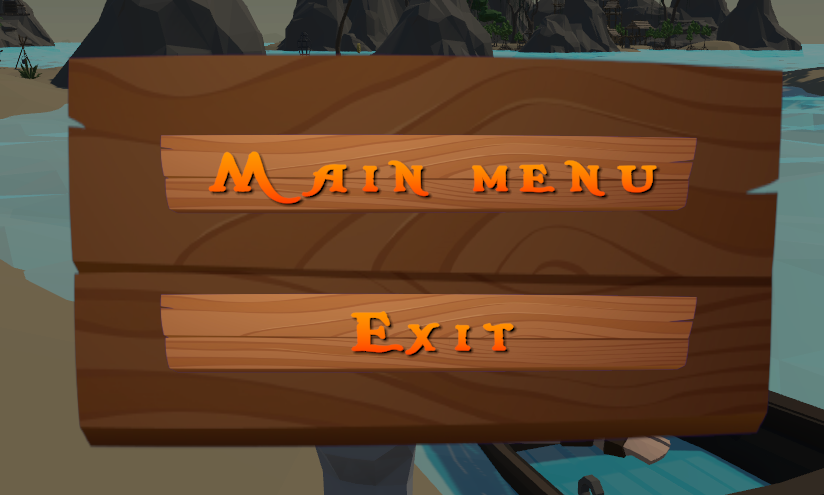
\includegraphics[width=.8\textwidth]{Figures/pauseUI.png}
	\caption{Ponuka s možnosťou návratu do hlavnej ponuky alebo ukončenia hry}
	\label{pic:PauseUI}
\end{figure}

Obe tlačidlá na UI elemente zobrazenom na obrázku \ref{pic:PauseUI} obsahujú Unity komponentu Button, ktorá vie napríklad zmeniť farebnú schému elementu, keď nad ním hráč nadíde myšou ale dôležitejšou funkcionalitou je event OnClick, ktorému je možné priamo v editore predať ľubovoľný objekt a tlačidlo na ňom dokáže zavolať určenú verejnú metódu, čo demonštruje obrázok \ref{pic:OnClick}. V tomto prípade bol tlačidlám predaný objekt GameManager a volané boli jeho dve verejné metódy OpenMainMenu() a QuitGame() zobrazené vo výpise \ref{src:MMQuit}. 

\begin{figure}[!htbp]
	\centering
	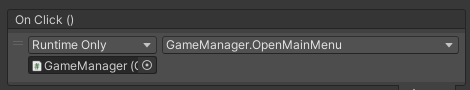
\includegraphics[width=.8\textwidth]{Figures/OnClick.png}
	\caption{Nastavenie OnClick eventu tlačidla v editore}
	\label{pic:OnClick}
\end{figure}

\vspace{8pt}
\begin{lstlisting}[label=src:MMQuit,caption={Metódy na návrat do hlavnej ponuky a ukončenie hry}]
public void OpenMainMenu()
    {
        SceneManager.LoadScene(0);
    }
    public void QuitGame()
    {
#if UNITY_EDITOR
        UnityEditor.EditorApplication.isPlaying = false;
#endif
        Application.Quit();
    }
\end{lstlisting}

Metóda OpenMainMenu() načíta scénu s build indexom 0. Tento postup je vhodné aplikovať, keď máme fixne dané poradie scén v zostavení aplikácie. Je to efektívnejšia metóda ako vyhľadávanie scény podľa mena. Poradie scén bolo popísané v sekcií \ref{sec:GameStructure}. 

Ukončenie hry potom prebieha jednoduchým zavolaním metódy Application.Quit(). Problém tohto prístupu spočíva v tom, že to nevypne hru bežiacu v rámci editora Unity. Z tohto dôvodu je v rámci direktivy preprocesoru UNITY\_EDITOR, nutné aj nastavenie premennej isPlaying v triede UnityEditor.EditorApplication na hodnotu false. Direktívy preprocesoru v C\# obecne umožňujú selektívne zahrnúť alebo vylúčiť kód z kompilácie na základe toho, či sú alebo nie sú definované určité skriptovacie symboly. Editor Unity ná na tieto účely preddefinované symboly pre rozlíšenie rôznych platforiem či práve zostavenia aplikácie od behu v editore \cite{ConditionalCompilation}.

Jednotlivé UI elementy či obrazovky sú v triedach referencované pomocou atribútu [SerializeField], ktorý vynúti serializáciu u neverejných členských premenných \cite{SerializeField}, čím sa neporušuje princíp zapuzdrenia a zároveň to umožňuje jednoducho referencovať medzi sebou objekty priamo v editore Unity pomocou metódy Drag & Drop či výberu z rolovacej ponuky. Nie je teda nutné prehľadávať objekty v scéne alebo riešiť prístup k danému objektu architektonicky na úrovni kódu. 

\subsection{Hlavná ponuka a užívateľské rozhranie}
\label{sec:MainMenuAndUI}
%TODO
%TODO
\subsection{Perzistentné nastavenia hry}
\label{sec:Settings}
%TODO + config manager

%TODO

\section{Štruktúra hráčskej postavy}
\label{sec:Player}
%TODO
\subsection{Ovládanie hry}
\label{sec:Input} %+ input manager + camera
%TODO
\section{Štruktúra NPC agentov}
\label{sec:Agents}
%TODO + enemy spawner
%NAVMESH
\subsection{Zmyslové vnímanie agentov}
\label{sec:Perception}
%TODO + soundManager + noise

% Chapter 5
\chapter{Rozhodovanie agentov s využitím rozhodovacích stromov}
\label{sec:ImplDecisionTrees}
%TODO
\section{Algoritmus ID3}
\label{sec:ID3}
%TODO
\section{Algoritmus D4.5}
\label{sec:D45}
%TODO
\section{Algoritmus CART}
\label{sec:CART}
%TODO

% Chapter 6
\chapter{Rozhodovanie agentov s využitím spätnoväzobného učenia}
\label{sec:ImplReinforcement learning}
%TODO
\section{Inštalácia prvotné nastavenie nástroja ML-Agents}
\label{sec:Agents}
%TODO
\section{Trénovanie agentov}
\label{sec:Training}
%TODO
\subsection{Prvý trénovací scenár}
\label{sec:FirstScenario}
%TODO
%...
\subsection{N-tý trénovací scenár}
\label{sec:LastScenario}
%TODO

% Chapter 7
\chapter{Porovnanie prístupov}
\label{sec:ImplReinforcement learning}
%TODO
\section{Porovnanie z hľadiska výkonu}
\label{sec:Performance}
%TODO
\section{Empirické porovnanie}
\label{sec:Gameplay}
%TODO

% Chapter 8
\chapter{Záver}
\label{sec:Conclusion}

%Template/Testing
\begin{figure}[!htbp]
	\centering
	
\includegraphics[width=.5\textwidth]{Figures/FEI_CZ.pdf}
	\caption{Test}
	\label{pic:Teeest}
\end{figure}

\begin{center}
\begin{tabular}{ c c c }
 cell1 & cell2 & cell3 \\ 
 cell4 & cell5 & cell6 \\  
 cell7 & cell8 & cell9    
\end{tabular}
\end{center}

\begin{lstlisting}[label=src:Test,caption={Test}]
// Hello World! program
namespace HelloWorld
{
    class Hello {         
        static void Main(string[] args)
        {
            System.Console.WriteLine("Hello World!");
        }
    }
}
\end{lstlisting}
%End of Template/Testing

% Prílohy
%\appendix
%\input{appendix_mono}

\printbibliography[title={Literatúra}, heading=bibintoc]
\end{document}
